%%%%%%%%%%%%%%%%%%%%%%%%%%%%%%%%%%%%%%%%%%%%%%%%%%%%%%%%%%%%%%%%%%%%%%%%%%%%%
\begin{frame}{Simulate agent behavior}\label{simulate}

% To consider how my model can explain human capital sepcialization decisions

How can the model explain different specialization outcomes?

\vspace{3ex}
Consider a world with two fields, X and Y
\begin{itemize}
    \item Wages are equal: $w_X = w_Y$
    \item The agent's probabilities of success are equal: $\theta_X = \theta_Y$
    \item Initial beliefs are equal to the uninformative prior: \hyperlink{model_beta_11}{\beamerbutton{PDF of beliefs}}
    \begin{equation*}
        (\alpha_{X0}, \beta_{X0}) = (\alpha_{Y0}, \beta_{Y0}) = (1, 1)
    \end{equation*}
\end{itemize}

\vspace{3ex}
Simulate agent's specialization decisions when choosing between X and Y
\begin{itemize}
    \item Model fraction of simulated agents choosing X or Y at time $t$ 
    \item Assume $h_{j0} = \nu \alpha_{j0}$ \hyperlink{sim_parameterization}{\beamerbutton{Details}}
\end{itemize}


\end{frame}

%%%%%%%%%%%%%%%%%%%%%%%%%%%%%%%%%%%%%%%%%%%%%%%%%%%%%%%%%%%%%%%%%%%%%%%%%%%%%%%%
\begin{frame}{Default parameterization}\label{sim_default}

% 
\begin{figure}
\centering
% This file was created by tikzplotlib v0.9.2.
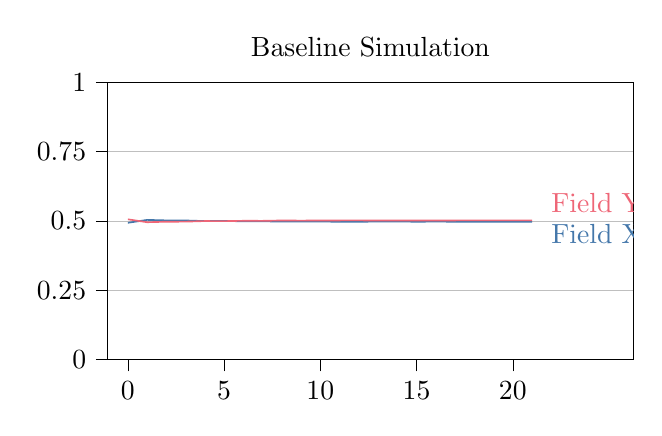
\begin{tikzpicture}

\definecolor{color0}{rgb}{0.266666666666667,0.466666666666667,0.666666666666667}
\definecolor{color1}{rgb}{0.933333333333333,0.4,0.466666666666667}

\begin{axis}[
height=5.101085673964669cm,
tick align=outside,
tick pos=left,
title={Baseline Simulation},
width=8.25373cm,
x grid style={white!69.0196078431373!black},
xmin=-1.05, xmax=26.25,
xtick style={color=black},
xtick={0,5,10,15,20},
xticklabels={\(\displaystyle 0\),\(\displaystyle 5\),\(\displaystyle 10\),\(\displaystyle 15\),\(\displaystyle 20\)},
ymajorgrids,
ymin=0, ymax=1,
ytick style={color=black},
ytick={0,0.25,0.5,0.75,1},
yticklabels={\(\displaystyle 0\),\(\displaystyle 0.25\),\(\displaystyle 0.5\),\(\displaystyle 0.75\),\(\displaystyle 1\)}
]
\addplot [semithick, color0]
table {%
0 0.4937
1 0.5042
2 0.5024
3 0.5021
4 0.5
5 0.5003
6 0.4991
7 0.4992
8 0.4979
9 0.4984
10 0.4979
11 0.4977
12 0.4976
13 0.498
14 0.498
15 0.4977
16 0.4979
17 0.4977
18 0.4976
19 0.4976
20 0.4976
21 0.4976
};
\addplot [semithick, color1]
table {%
0 0.5063
1 0.4958
2 0.4976
3 0.4979
4 0.5
5 0.4997
6 0.5009
7 0.5008
8 0.5021
9 0.5016
10 0.5021
11 0.5023
12 0.5024
13 0.502
14 0.502
15 0.5023
16 0.5021
17 0.5023
18 0.5024
19 0.5024
20 0.5024
21 0.5024
};
\draw (axis cs:21.5,0.4176) node[
  anchor=base west,
  text=color0,
  rotate=0.0
]{Field X};
\draw (axis cs:21.5,0.5324) node[
  anchor=base west,
  text=color1,
  rotate=0.0
]{Field Y};
\end{axis}

\end{tikzpicture}

\end{figure}

\hyperlink{model_beta_11}{\beamerbutton{PDF of beliefs}}
\end{frame}

%%%%%%%%%%%%%%%%%%%%%%%%%%%%%%%%%%%%%%%%%%%%%%%%%%%%%%%%%%%%%%%%%%%%%%%%%%%%%%%%
\begin{frame}{Zooming in}

% should be symmetric

\begin{figure}
\centering
% This file was created by tikzplotlib v0.9.2.
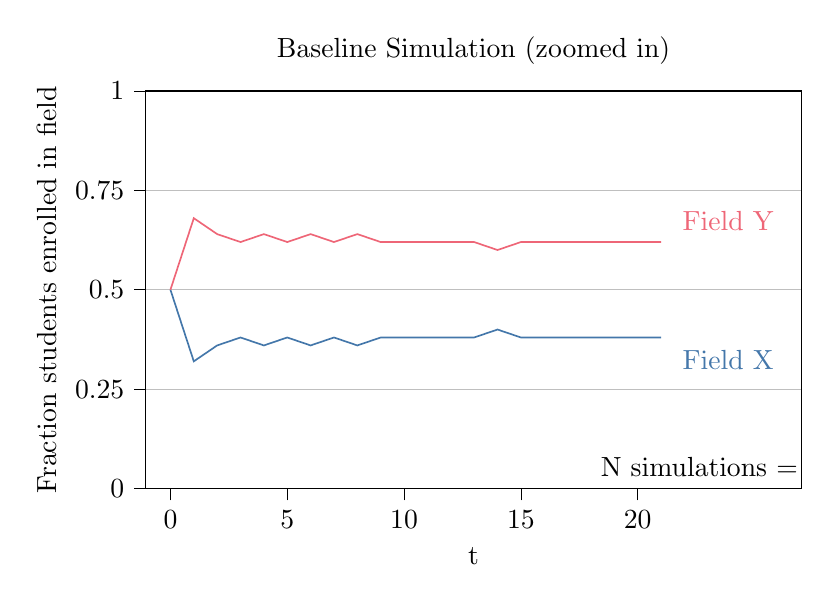
\begin{tikzpicture}

\definecolor{color0}{rgb}{0.266666666666667,0.466666666666667,0.666666666666667}
\definecolor{color1}{rgb}{0.933333333333333,0.4,0.466666666666667}

\begin{axis}[
height=6.6314113761540705cm,
tick align=outside,
tick pos=left,
title={Baseline Simulation (zoomed in)},
width=9.904475999999999cm,
x grid style={white!69.0196078431373!black},
xlabel={t},
xmin=-1.05, xmax=27,
xtick style={color=black},
xtick={0,5,10,15,20},
xticklabels={\(\displaystyle 0\),\(\displaystyle 5\),\(\displaystyle 10\),\(\displaystyle 15\),\(\displaystyle 20\)},
ylabel={Fraction students enrolled in field},
ymajorgrids,
ymin=0, ymax=1,
ytick style={color=black},
ytick={0,0.25,0.5,0.75,1},
yticklabels={\(\displaystyle 0\),\(\displaystyle 0.25\),\(\displaystyle 0.5\),\(\displaystyle 0.75\),\(\displaystyle 1\)}
]
\addplot [semithick, color0]
table {%
0 0.5
1 0.319999933242798
2 0.360000014305115
3 0.379999995231628
4 0.360000014305115
5 0.379999995231628
6 0.360000014305115
7 0.379999995231628
8 0.360000014305115
9 0.379999995231628
13 0.379999995231628
14 0.399999976158142
15 0.379999995231628
21 0.379999995231628
};
\addplot [semithick, color1]
table {%
0 0.5
1 0.680000066757202
2 0.639999985694885
3 0.620000004768372
4 0.639999985694885
5 0.620000004768372
6 0.639999985694885
7 0.620000004768372
8 0.639999985694885
9 0.620000004768372
13 0.620000004768372
14 0.600000023841858
15 0.620000004768372
21 0.620000004768372
};
\draw (axis cs:21.5,0.3) node[
  anchor=base west,
  text=color0,
  rotate=0.0
]{Field X};
\draw (axis cs:21.5,0.65) node[
  anchor=base west,
  text=color1,
  rotate=0.0
]{Field Y};
\draw (axis cs:18,0.03) node[
  anchor=base west,
  text=black,
  rotate=0.0
]{N simulations = 50};
\end{axis}

\end{tikzpicture}

\end{figure}


\end{frame}

%%%%%%%%%%%%%%%%%%%%%%%%%%%%%%%%%%%%%%%%%%%%%%%%%%%%%%%%%%%%%%%%%%%%%%%%%%%%%%%%
\begin{frame}{Wage effects}

% 

\begin{figure}
\centering
% This file was created by tikzplotlib v0.9.2.
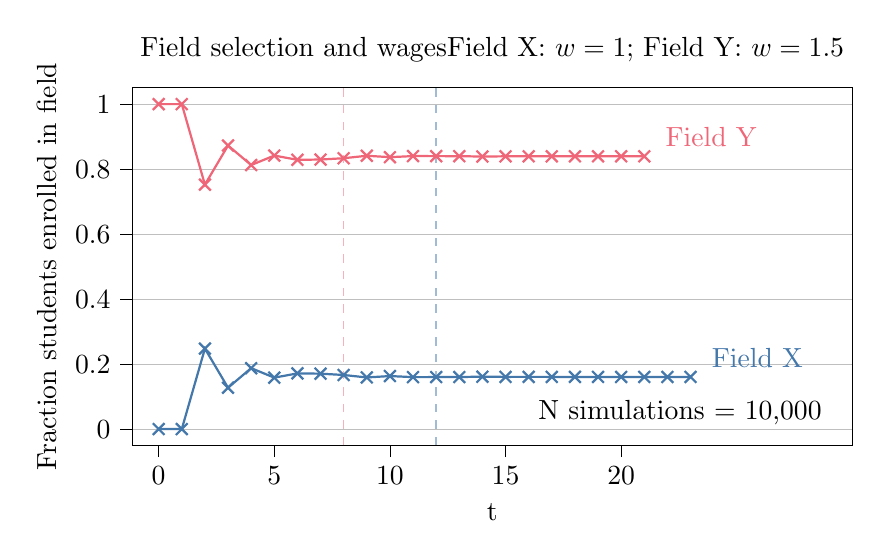
\begin{tikzpicture}

\definecolor{color0}{rgb}{0.266666666666667,0.466666666666667,0.666666666666667}
\definecolor{color1}{rgb}{0.933333333333333,0.4,0.466666666666667}

\begin{axis}[
height=6.121302808757603cm,
tick align=outside,
tick pos=left,
title={Field selection and wages  \\ Field X: \(\displaystyle w = 1\); Field Y: \(\displaystyle w = 1.5\)},
unbounded coords=jump,
width=10.729849cm,
x grid style={white!69.0196078431373!black},
xlabel={t},
xmin=-1.15, xmax=30,
xtick style={color=black},
xtick={0,5,10,15,20},
xticklabels={\(\displaystyle 0\),\(\displaystyle 5\),\(\displaystyle 10\),\(\displaystyle 15\),\(\displaystyle 20\)},
ylabel={Fraction students enrolled in field},
ymajorgrids,
ymin=-0.05, ymax=1.05,
ytick style={color=black},
ytick={0,0.2,0.4,0.6,0.8,1},
yticklabels={\(\displaystyle 0\),\(\displaystyle 0.2\),\(\displaystyle 0.4\),\(\displaystyle 0.6\),\(\displaystyle 0.8\),\(\displaystyle 1\)}
]
\addplot [thick, color0, mark=x, mark size=3, mark options={solid}]
table {%
0 0
1 0
2 0.2477
3 0.1273
4 0.1875
5 0.1583
6 0.1714
7 0.1705
8 0.1665
9 0.1589
10 0.1632
11 0.1599
12 0.16
13 0.1602
14 0.1613
15 0.1606
16 0.1607
17 0.1606
18 0.1606
19 0.1605
20 0.1605
21 0.1605
22 0.1605
23 0.1605
};
\addplot [thick, color1, mark=x, mark size=3, mark options={solid}]
table {%
0 1
1 1
2 0.7523
3 0.8727
4 0.8125
5 0.8417
6 0.8286
7 0.8295
8 0.8335
9 0.8411
10 0.8368
11 0.8401
12 0.84
13 0.8398
14 0.8387
15 0.8394
16 0.8393
17 0.8394
18 0.8394
19 0.8395
20 0.8395
21 0.8395
22 nan
23 nan
};
\addplot [semithick, color0, opacity=0.5, dashed]
table {%
12 -0.05
12 1.05
};
\addplot [semithick, color1, opacity=0.5, dashed]
table {%
8 -0.05
8 1.05
};
\draw (axis cs:23.5,0.1905) node[
  anchor=base west,
  text=color0,
  rotate=0.0
]{Field X};
\draw (axis cs:21.5,0.8695) node[
  anchor=base west,
  text=color1,
  rotate=0.0
]{Field Y};
\draw (axis cs:16,0.03) node[
  anchor=base west,
  text=black,
  rotate=0.0
]{N simulations = 10,000};
\end{axis}

\end{tikzpicture}

\end{figure}

\end{frame}

%%%%%%%%%%%%%%%%%%%%%%%%%%%%%%%%%%%%%%%%%%%%%%%%%%%%%%%%%%%%%%%%%%%%%%%%%%%%%%%%
\begin{frame}{Belief effects}\label{sim_beliefs}

% risk aspect is on human capital accumulation
% your expected probability of gaining human capital is the same in both of these
% there's risk in timing - risk aversion over time; probably from discounting with linear utility function

%%%%%%%%%%%%
% Start going into y because you have more information
% more quickly will converge into what you go at 

% If you'er going to switch, you know sooner

% In expectation 
% What drives length to degree?
% AFter two periods you have sunk benefit


% Inforamtion value outweight human capital
% risk neutral is human capital 

% spend more in uncertain major 

% benefit 

% why do you spend less time studying when you  have more certainty

% if distribution is tighter, initial 

% any signal makes you more likely to switch if you start in more dispersed prior
% swtiching is bad; want to minimize time you spend in school
% go with option for which you 

% c_j depends on alpha0 and beta0

% poteriro vs posterior predictive

% Y provides more 
% you want to accumulate the most human capital in the shortest amount of time
% want to choose the field to get you to 10 suc

\begin{figure}
\centering
% This file was created by tikzplotlib v0.9.2.
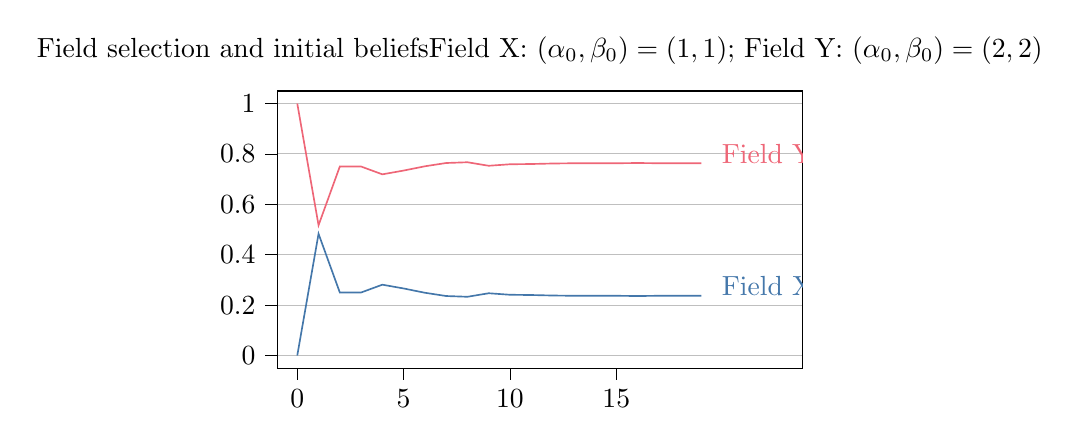
\begin{tikzpicture}

\definecolor{color0}{rgb}{0.266666666666667,0.466666666666667,0.666666666666667}
\definecolor{color1}{rgb}{0.933333333333333,0.4,0.466666666666667}

\begin{axis}[
height=5.101085673964669cm,
tick align=outside,
tick pos=left,
title={Field selection and initial beliefs \\ Field X: \(\displaystyle (\alpha_0, \beta_0)=(1, 1)\); Field Y: \(\displaystyle (\alpha_0, \beta_0)=(2, 2)\)},
width=8.25373cm,
x grid style={white!69.0196078431373!black},
xmin=-0.95, xmax=23.75,
xtick style={color=black},
xtick={0,5,10,15},
xticklabels={\(\displaystyle 0\),\(\displaystyle 5\),\(\displaystyle 10\),\(\displaystyle 15\)},
ymajorgrids,
ymin=-0.05, ymax=1.05,
ytick style={color=black},
ytick={0,0.2,0.4,0.6,0.8,1},
yticklabels={\(\displaystyle 0\),\(\displaystyle 0.2\),\(\displaystyle 0.4\),\(\displaystyle 0.6\),\(\displaystyle 0.8\),\(\displaystyle 1\)}
]
\addplot [semithick, color0]
table {%
0 0
1 0.483
2 0.25
3 0.25
4 0.281
5 0.266
6 0.249
7 0.236
8 0.233
9 0.247
10 0.241
11 0.24
12 0.238
13 0.237
14 0.237
15 0.237
16 0.236
17 0.237
18 0.237
19 0.237
};
\addplot [semithick, color1]
table {%
0 1
1 0.517
2 0.75
3 0.75
4 0.719
5 0.734
6 0.751
7 0.764
8 0.767
9 0.753
10 0.759
11 0.76
12 0.762
13 0.763
14 0.763
15 0.763
16 0.764
17 0.763
18 0.763
19 0.763
};
\draw (axis cs:19.5,0.237) node[
  anchor=base west,
  text=color0,
  rotate=0.0
]{Field X};
\draw (axis cs:19.5,0.763) node[
  anchor=base west,
  text=color1,
  rotate=0.0
]{Field Y};
\end{axis}

\end{tikzpicture}

\end{figure}
\hyperlink{model_beta_22}{\beamerbutton{PDF of beliefs}}
\hyperlink{sim_parameterization}{\beamerbutton{Parameterization}}
\hyperlink{app_ability_v_effect}{\beamerbutton{
    Let $\alpha_{X0} \nu_X = \alpha_{Y0} \nu_Y$
}}

\end{frame}

%%%%%%%%%%%%%%%%%%%%%%%%%%%%%%%%%%%%%%%%%%%%%%%%%%%%%%%%%%%%%%%%%%%%%%%%%%%%%%%%
\begin{frame}{Ability to succeed}\label{sim_ability}

\begin{figure}
\centering
% This file was created by tikzplotlib v0.9.1.
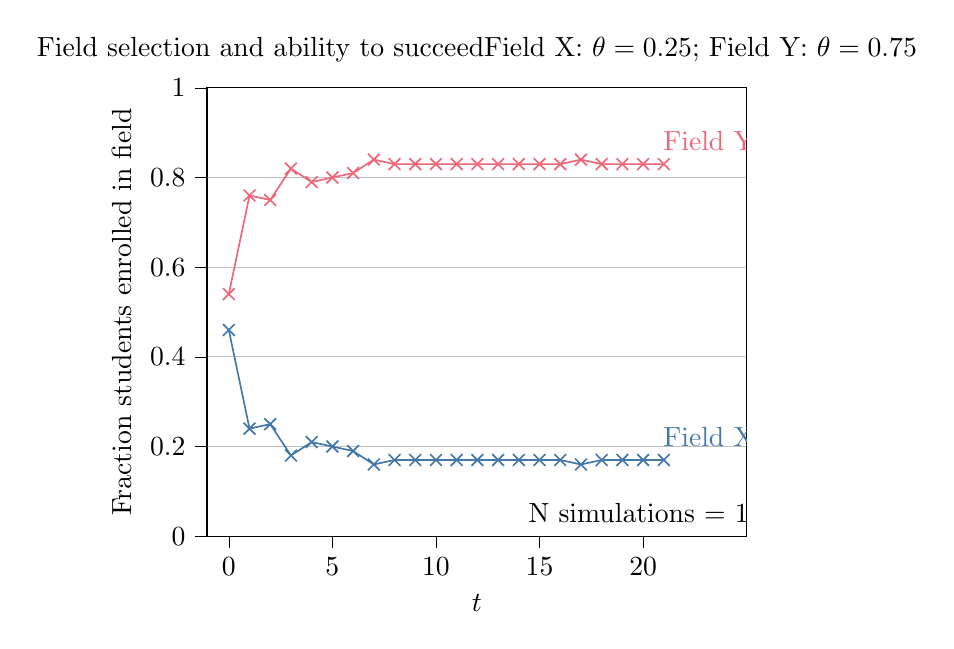
\begin{tikzpicture}

\definecolor{color0}{rgb}{0.266666666666667,0.466666666666667,0.666666666666667}
\definecolor{color1}{rgb}{0.933333333333333,0.4,0.466666666666667}

\begin{axis}[
height=207pt,
tick align=outside,
tick pos=left,
title={Field selection and ability to succeed \\ Field X: \(\displaystyle \theta=0.25\); Field Y: \(\displaystyle \theta=0.75\)},
width=240pt,
x grid style={white!69.0196078431373!black},
xlabel={\(\displaystyle t\)},
xmin=-1.05, xmax=25,
xtick style={color=black},
xtick={0,5,10,15,20},
xticklabels={\(\displaystyle 0\),\(\displaystyle 5\),\(\displaystyle 10\),\(\displaystyle 15\),\(\displaystyle 20\)},
ylabel={Fraction students enrolled in field},
ymajorgrids,
ymin=0, ymax=1,
ytick style={color=black},
ytick={0,0.2,0.4,0.6,0.8,1},
yticklabels={\(\displaystyle 0\),\(\displaystyle 0.2\),\(\displaystyle 0.4\),\(\displaystyle 0.6\),\(\displaystyle 0.8\),\(\displaystyle 1\)}
]
\addplot [semithick, color0, mark=x, mark size=3, mark options={solid}]
table {%
0 0.46
1 0.24
2 0.25
3 0.18
4 0.21
5 0.2
6 0.19
7 0.16
8 0.17
9 0.17
10 0.17
11 0.17
12 0.17
13 0.17
14 0.17
15 0.17
16 0.17
17 0.16
18 0.17
19 0.17
20 0.17
21 0.17
};
\addplot [semithick, color1, mark=x, mark size=3, mark options={solid}]
table {%
0 0.54
1 0.76
2 0.75
3 0.82
4 0.79
5 0.8
6 0.81
7 0.84
8 0.83
9 0.83
10 0.83
11 0.83
12 0.83
13 0.83
14 0.83
15 0.83
16 0.83
17 0.84
18 0.83
19 0.83
20 0.83
21 0.83
};
\draw (axis cs:20.5,0.2) node[
  anchor=base west,
  text=color0,
  rotate=0.0
]{Field X};
\draw (axis cs:20.5,0.86) node[
  anchor=base west,
  text=color1,
  rotate=0.0
]{Field Y};
\draw (axis cs:14,0.03) node[
  anchor=base west,
  text=black,
  rotate=0.0
]{N simulations = 100};
\end{axis}

\end{tikzpicture}

\end{figure}
\hyperlink{app_v_effects}{\beamerbutton{$\nu$ simulation}}

\end{frame}